\section{Основная часть}

    \subsection{Описание модели}

        Одна из вариаций модели Хасселя имеет следующую математическая запись:

        \[x_{t+1} = \frac{\alpha x_t^2}{(\beta + x_t)^6}\]

        В данной формуле \(x_i\) --- количество особей в поколении с номером i. Параметр \(\alpha\) определяет скорость роста популяции, а параметр \(\beta\) определяет несущую способность окружающей среды.
    
    \subsection{Частный случай}
    
        Для упрощения задачи рассмотрим частный случай. Зафиксируем параметр \(\alpha = 1\). Параметр \(\beta\) изменяется в диапазоне \([0; 0.6]\). Теперь запишем уравнение в таком виде:

        \[x = \frac{\alpha x^2}{(\beta + x)^6}\]
    
        \[1 = \frac{\alpha x}{(\beta + x)^6}\]

        \[
            \tag{1}
            \label{baseEquation}
            \alpha x = (\beta + x)^6
        \]

        Данную формулу можно рассмотреть как две функции. Построим графики функций \(y = \alpha x\) и \(y = (\beta + x)^6\). 
        
        В зависимости от значений параметра \(\beta\) уравнение (\ref{baseEquation}) может иметь ноль, один или два корня. На рисунках (\ref{mainIntersect}), (\ref{mainTouch}) и (\ref{mainOver}) можно увидеть все возможные варианты.
        
        \begin{figure}
            \centering
            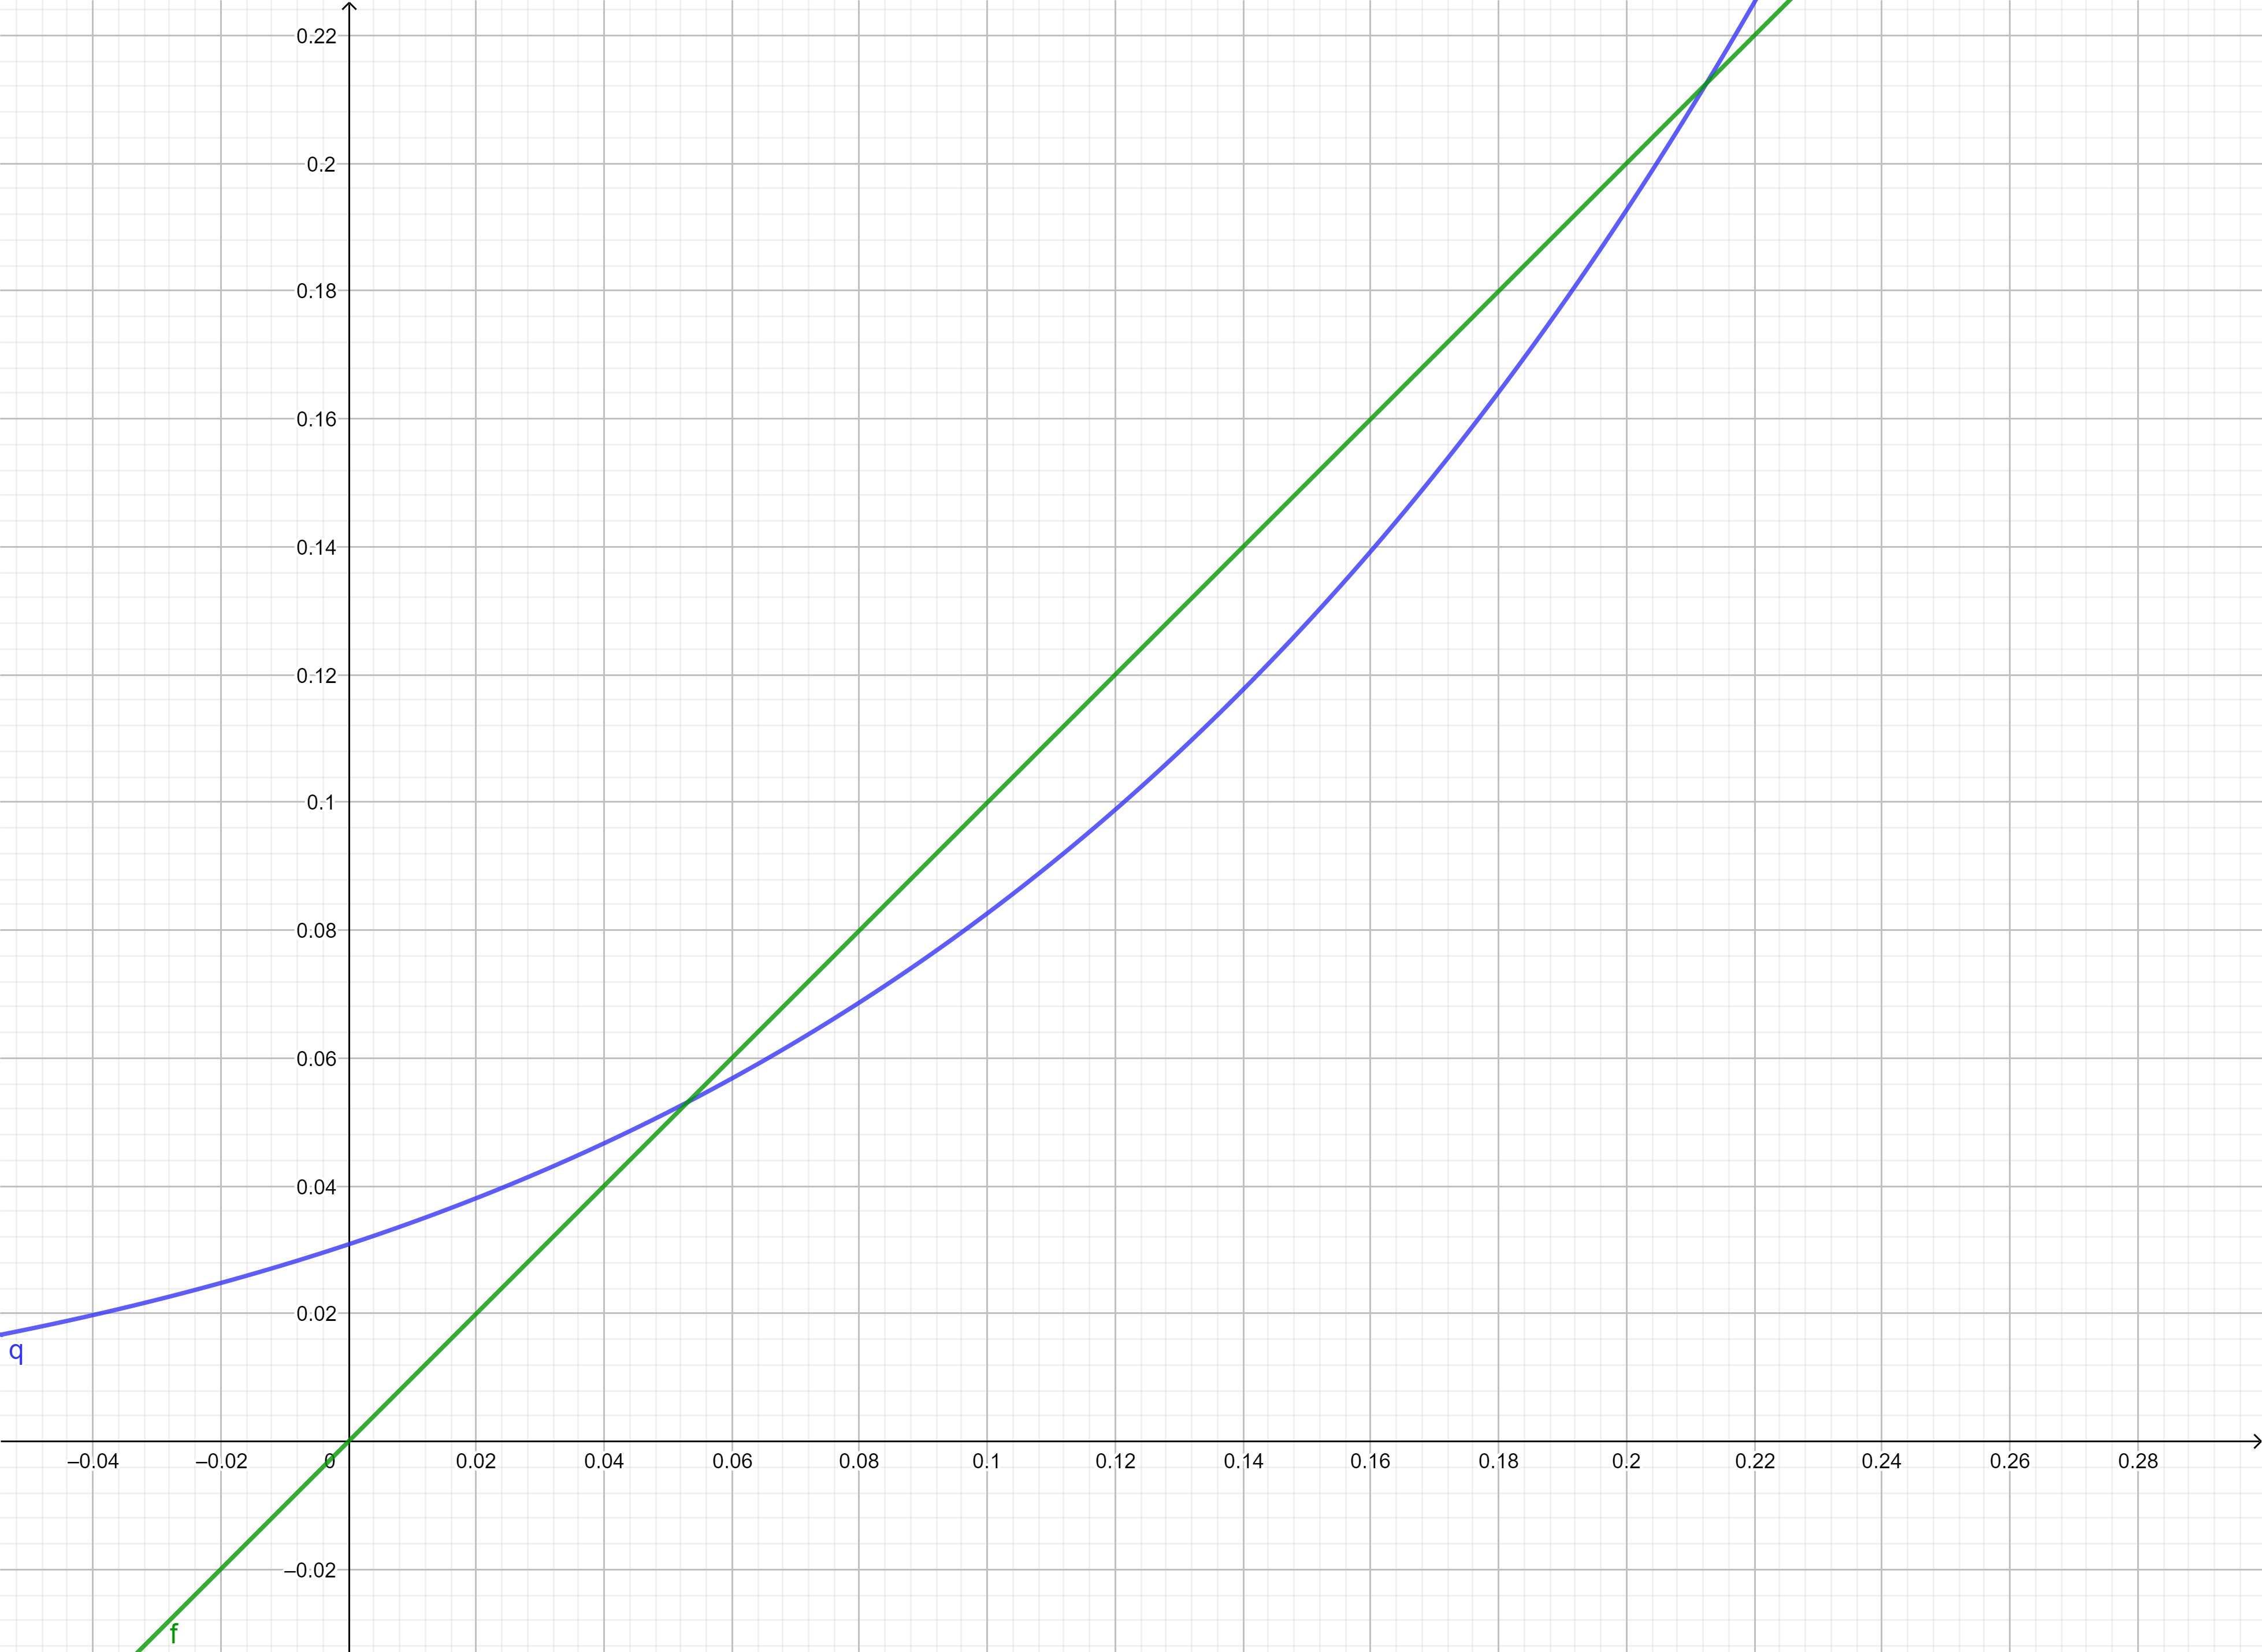
\includegraphics[width=0.75\textwidth]{images/main_intersect.jpg}

            \captionsetup{justification=centering}
            \caption{\(\beta < 0.582355932\)}
            \label{mainIntersect}
        \end{figure}

        \begin{figure}
            \centering
            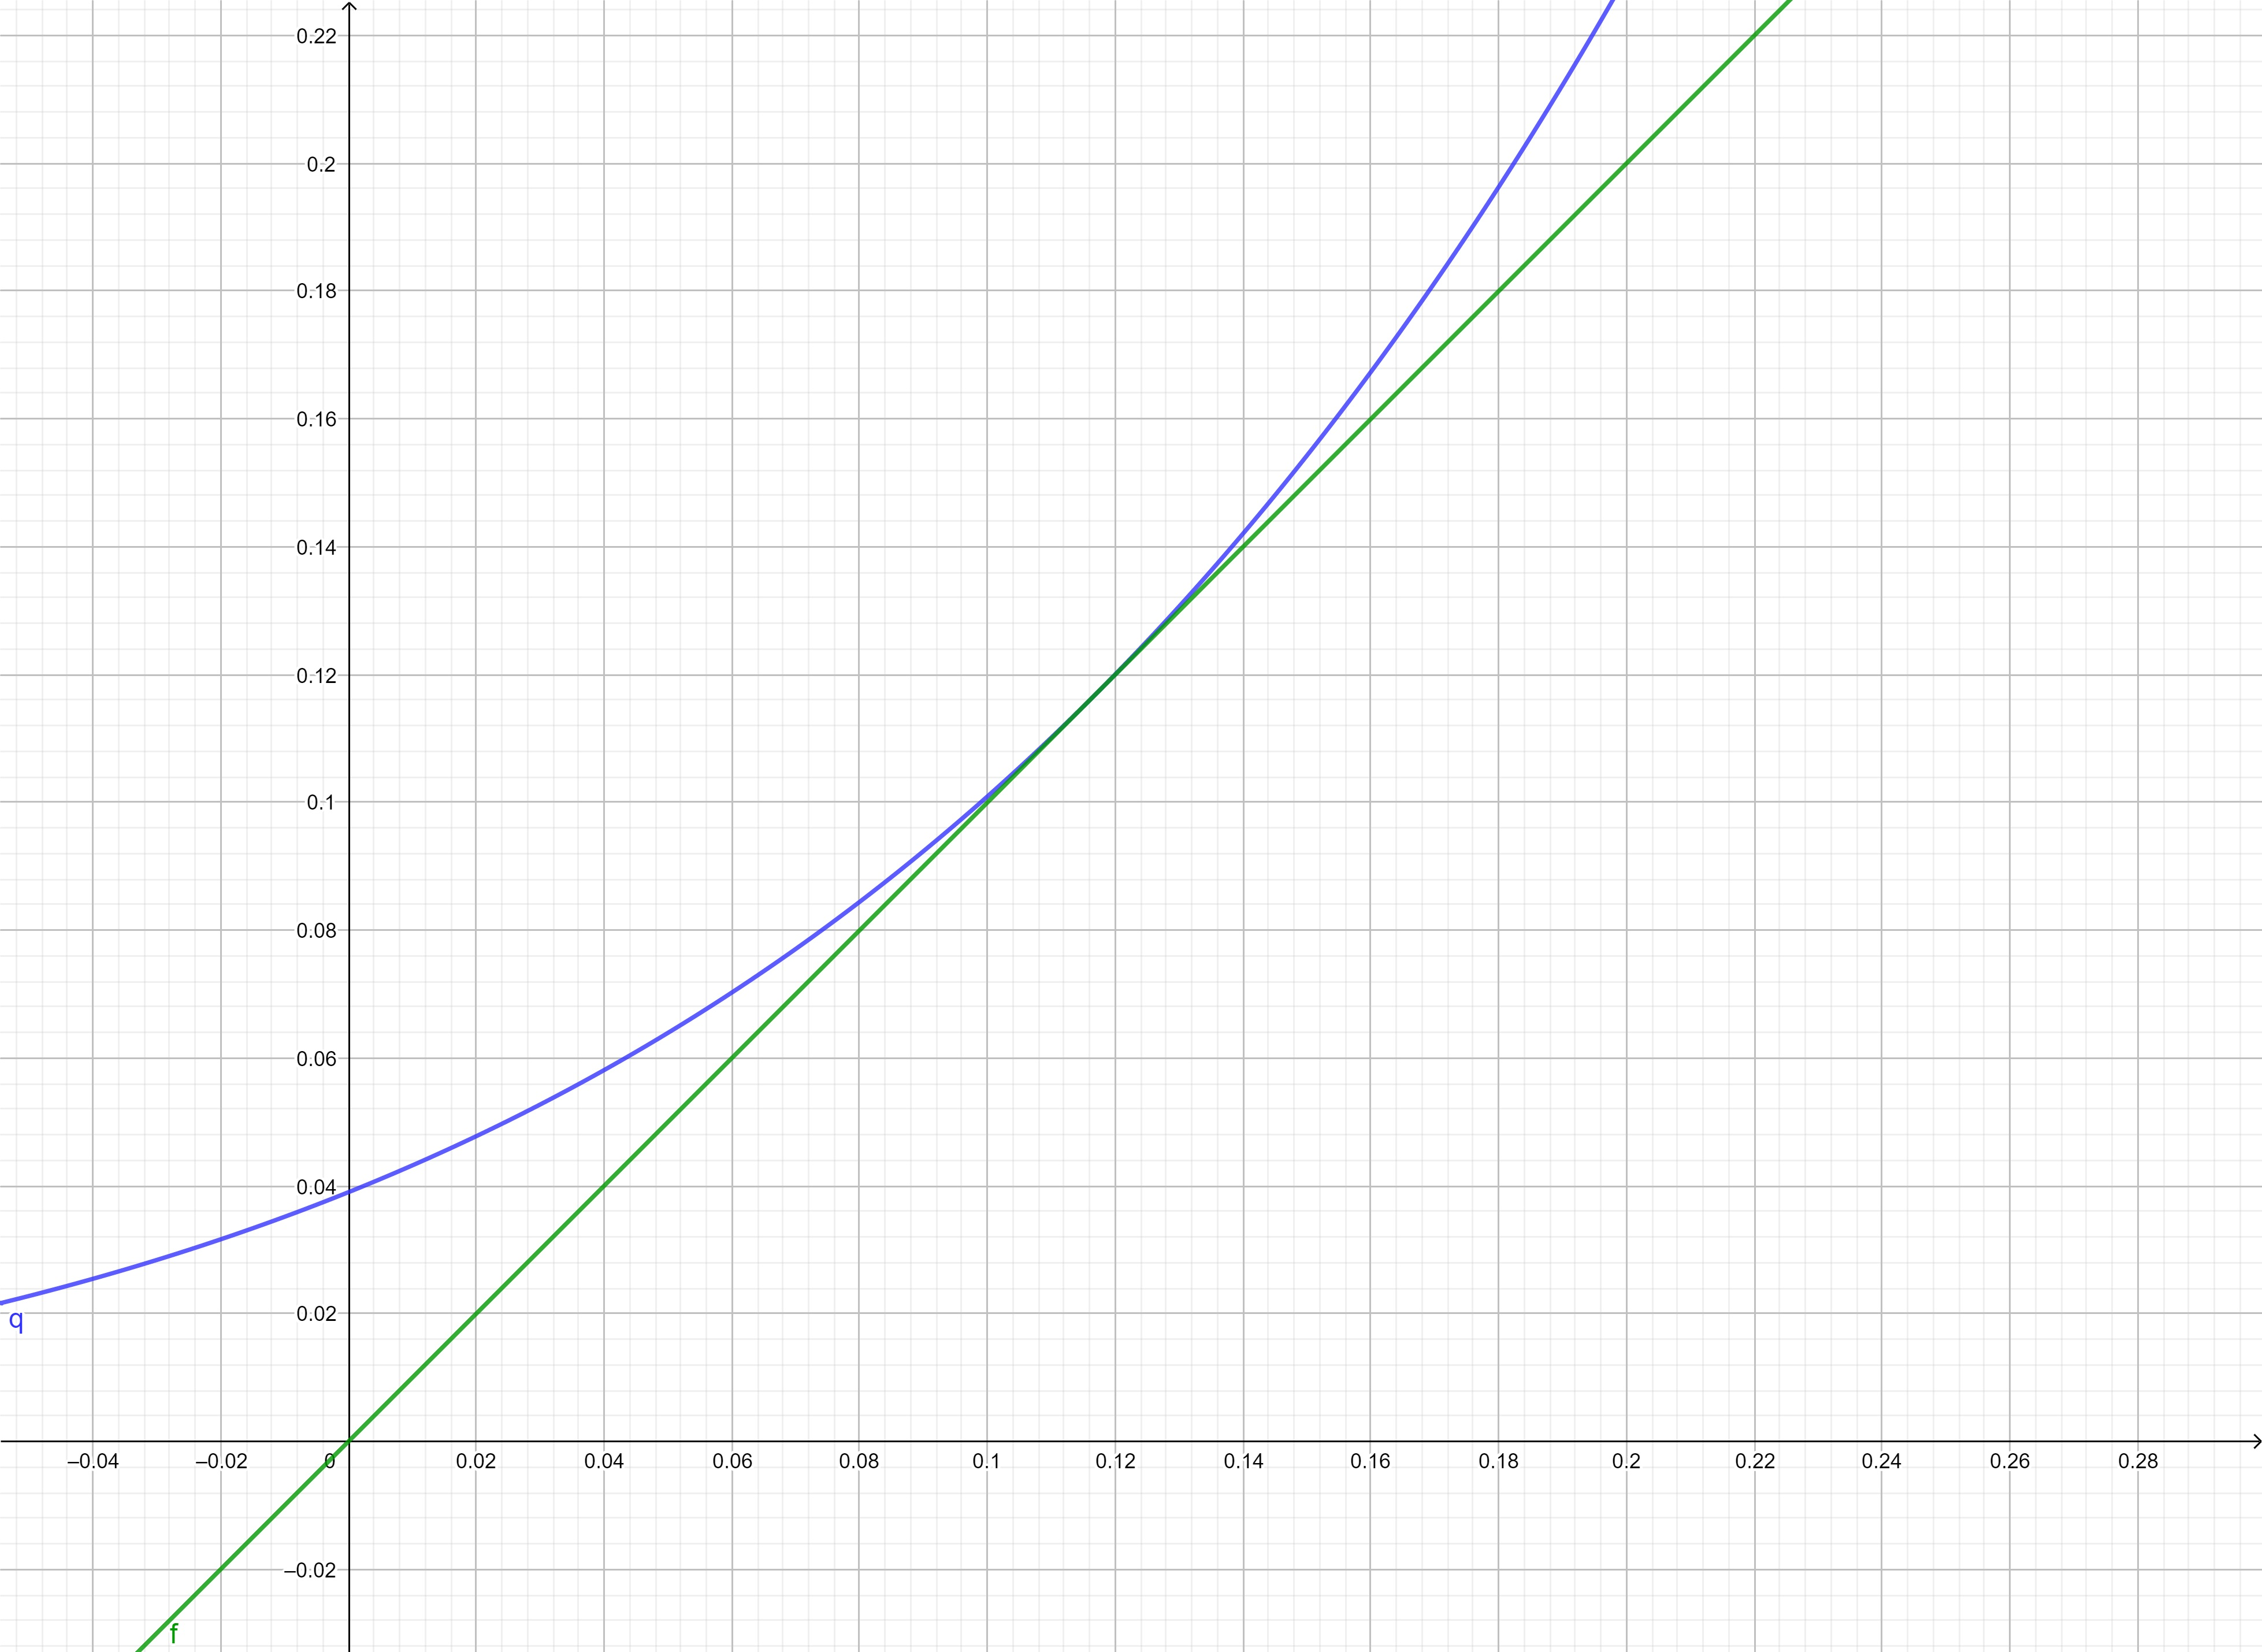
\includegraphics[width=0.75\textwidth]{images/main_touch.jpg}

            \captionsetup{justification=centering}
            \caption{\(\beta \approx 0.582355932\)}
            \label{mainTouch}
        \end{figure}

        \begin{figure}
            \centering
            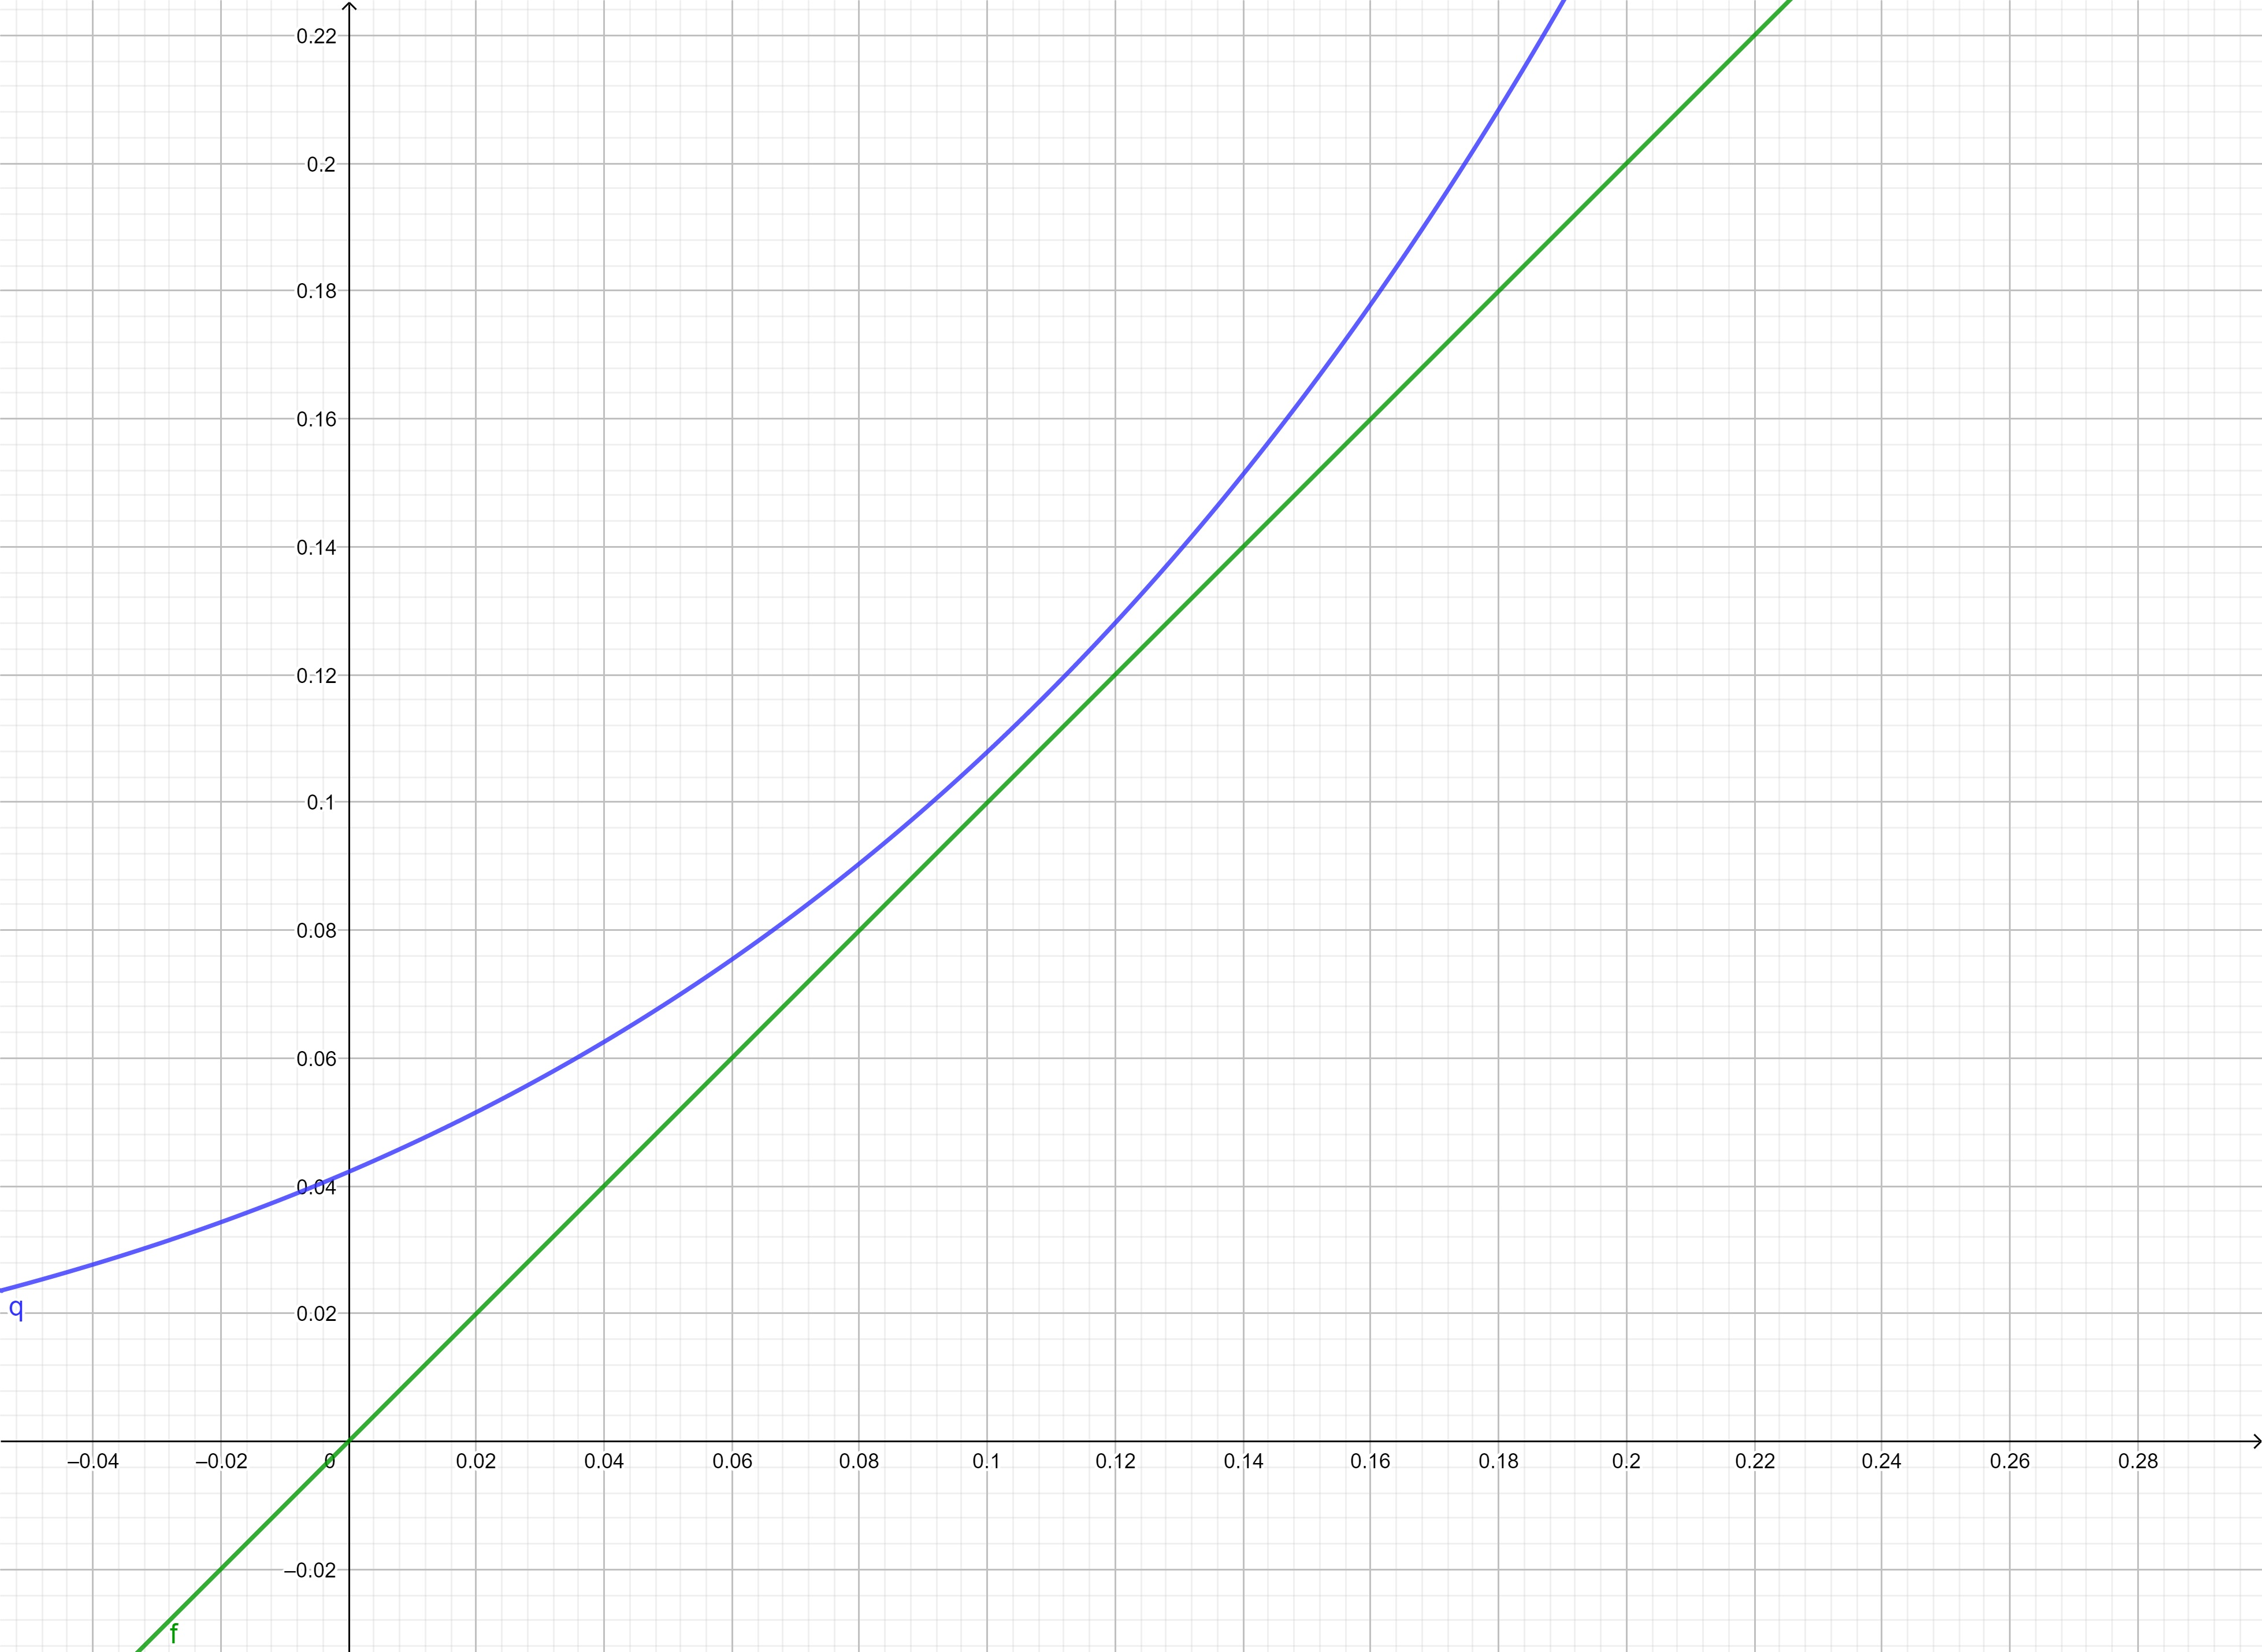
\includegraphics[width=0.75\textwidth]{images/main_over.jpg}

            \captionsetup{justification=centering}
            \caption{\(\beta > 0.582355932\)}
            \label{mainOver}
        \end{figure}

    \subsection{Временные ряды}

        Для анализа этой системы можно использовать временные ряды. Временной ряд позволяет наглядно показать как с течением времени изменяется численность популяции.

        Далее рассмотрим подробнее все возможные ситуации. Для этого давайте зафиксируем параметр следующим образом: \(\beta = 0.56\). 

        Давайте зафикисируем начальную численность популяции \(x_0 = 0.04\). На графике (\ref{time_series_x_0_04_b_0_56}) мы видим, что временной ряд сходится к нулю. В биологическом смысле это означает, что популяция с теченеим времени вымирает.
    
        \begin{figure}
            \centering
            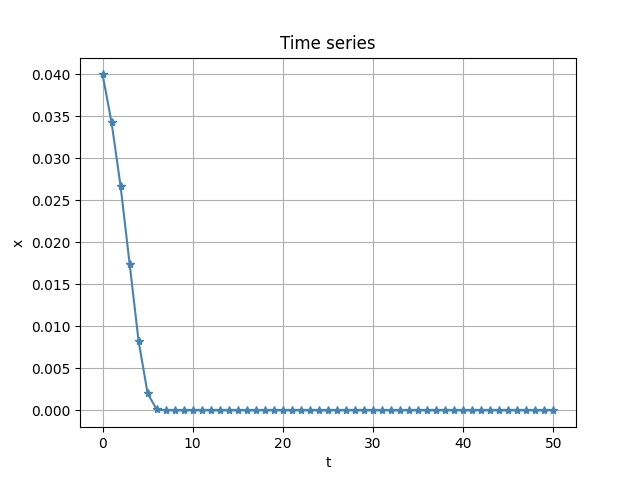
\includegraphics[width=0.75\textwidth]{time_series_x_0_04_b_0_56.jpg}

            \captionsetup{justification=centering}
            \caption{\(x_0 = 0.04; \beta = 0.56\)}
            \label{time_series_x_0_04_b_0_56}
        \end{figure}

        А теперь зафиксируем начальную численность популяции на уровне \(x_0 = 0.06\). На графике (\ref{time_series_x_0_06_b_0_56}) видно, что при таких начальных условиях популяция очень быстро увеличивается до некоторого предела. После достижения данного предела рост численности популяции прекращается. То есть популяция с течением времени стабилизируется.
    
        \begin{figure}
            \centering
            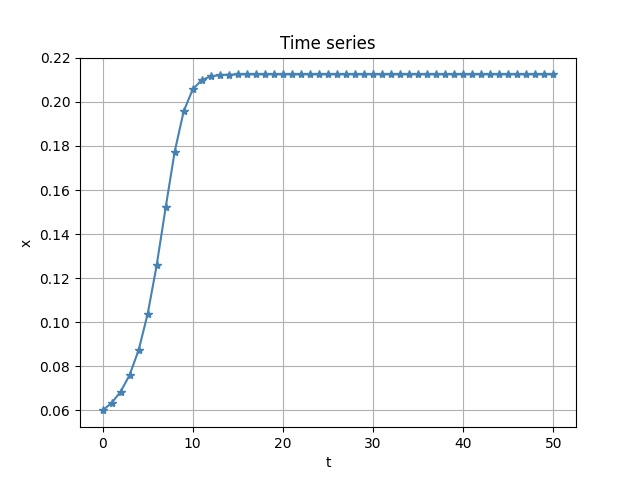
\includegraphics[width=0.75\textwidth]{time_series_x_0_06_b_0_56.jpg}

            \captionsetup{justification=centering}
            \caption{\(x_0 = 0.06; \beta = 0.56\)}
            \label{time_series_x_0_06_b_0_56}
        \end{figure}

        Очень похожую ситуацию мы можем наблюдать на графике (\ref{time_series_x_0_3_b_0_56}). Такой график построен при начальном значении \(x_0 = 0.3\). Значения численности популяции тоже сходятся к устойчивому равновесию. Численность снова стабилизируется.
    
        \begin{figure}
            \centering
            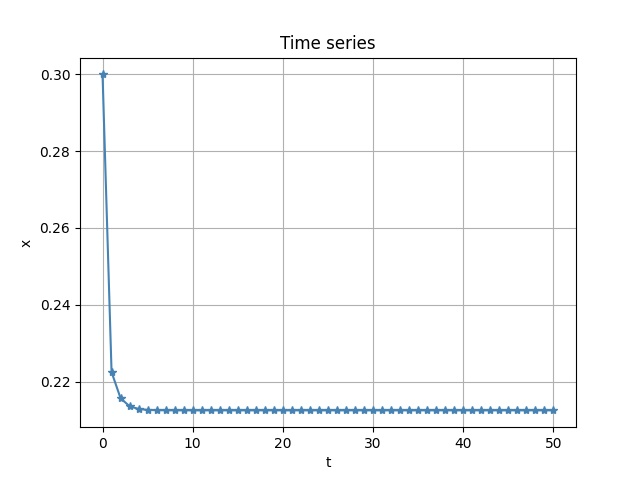
\includegraphics[width=0.75\textwidth]{time_series_x_0_3_b_0_56.jpg}

            \captionsetup{justification=centering}
            \caption{\(x_0 = 0.3; \beta = 0.56\)}
            \label{time_series_x_0_3_b_0_56}
        \end{figure}

        Теперь рассмотрим ситуацию, когда начальная численность популяции очень большая. Такая ситуация изображена на графике (\ref{time_series_x_1_2_b_0_56}). Мы видим, что происходит вымирание.
    
        \begin{figure}
            \centering
            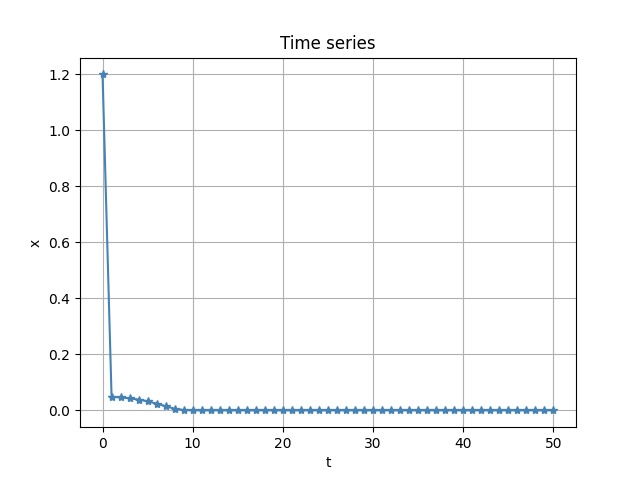
\includegraphics[width=0.75\textwidth]{time_series_x_1_2_b_0_56.jpg}

            \captionsetup{justification=centering}
            \caption{\(x_0 = 1.2; \beta = 0.56\)}
            \label{time_series_x_1_2_b_0_56}
        \end{figure}

    \subsection{Лестница Ламери}
    
        Существует также метод исследования называемый лестницой Ламери. Этот метод аналогично временному ряду позволяет выяснить к какому значению сходится значение популяции.
            
        Опять же рассмотрим подробнее все возможные ситуации. Для этого зафиксируем параметр: \(\beta = 0.56\). 
    
        Давайте зафикисируем начальную численность популяции \(x_0 = 0.04\). На графике (\ref{lamerei_x_0_04_b_0_56}) мы видим, что летсница Ламери сходится к нулю. В биологическом смысле это означает, что популяция с теченеим времени вымирает.
    
        \begin{figure}
            \centering
            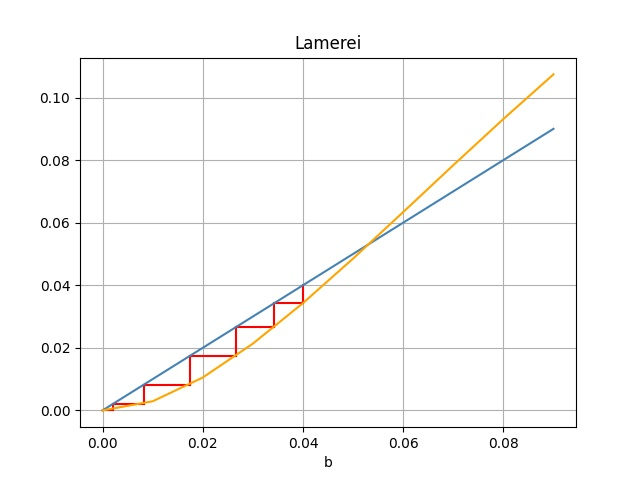
\includegraphics[width=0.75\textwidth]{lamerei_x_0_04_b_0_56.jpg}
    
            \captionsetup{justification=centering}
            \caption{\(x_0 = 0.04\)}
            \label{lamerei_x_0_04_b_0_56}
        \end{figure}
    
        А теперь зафиксируем начальную численность популяции на уровне \(x_0 = 0.06\). На графике (\ref{lamerei_x_0_06_b_0_56}) видно, что при таких начальных условиях численность популяции сходится к \(x \approx 0.21\).
            
        \begin{figure}
            \centering
            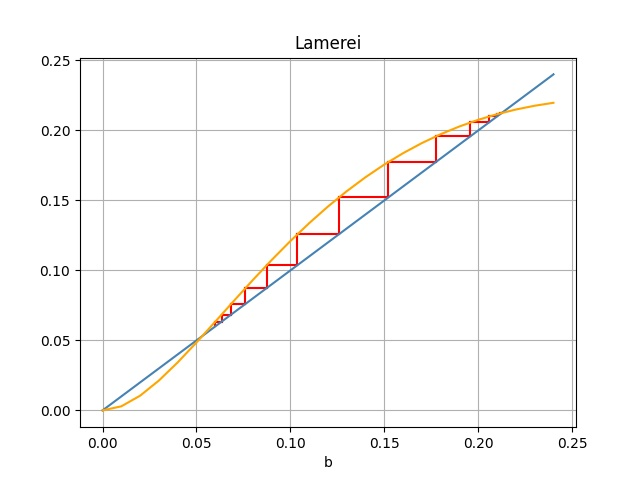
\includegraphics[width=0.75\textwidth]{lamerei_x_0_06_b_0_56.jpg}
    
            \captionsetup{justification=centering}
            \caption{\(x_0 = 0.06\)}
            \label{lamerei_x_0_06_b_0_56}
        \end{figure}
    
        Очень похожую ситуацию мы можем наблюдать на графике (\ref{lamerei_x_0_3_b_0_56}). Такой график построен при начальном значении \(x_0 = 0.3\). Значения численности популяции тоже сходятся к устойчивому равновесию. Численность снова стабилизируется.
            
        \begin{figure}
            \centering
            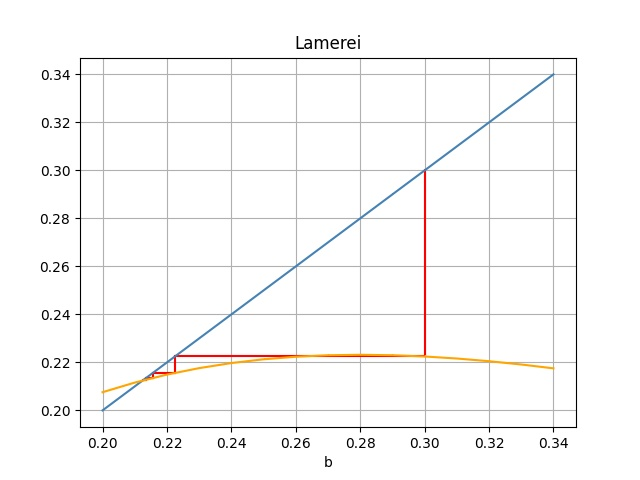
\includegraphics[width=0.75\textwidth]{lamerei_x_0_3_b_0_56.jpg}
    
            \captionsetup{justification=centering}
            \caption{\(x_0 = 0.3\)}
            \label{lamerei_x_0_3_b_0_56}
        \end{figure}
    
        Теперь рассмотрим ситуацию, когда начальная численность популяции очень большая. Такая ситуация изображена на графиках (\ref{lamerei_x_1_3_b_0_56}) и (\ref{lamerei2_x_1_3_b_0_56}). Мы видим, что опятьже происходит вымирание.
            
        \begin{figure}
            \centering
            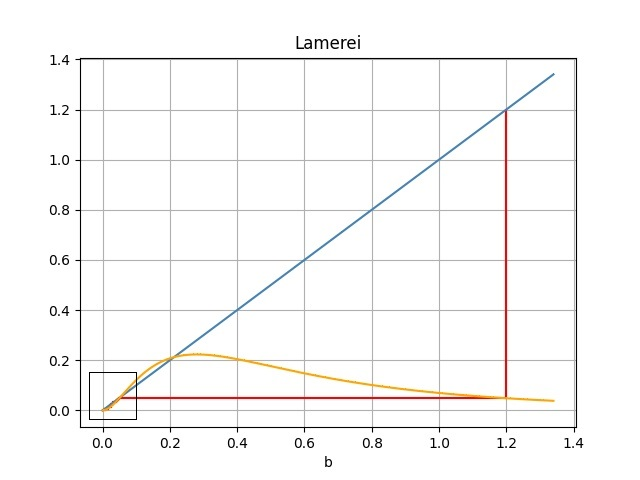
\includegraphics[width=0.75\textwidth]{lamerei_x_1_3_b_0_56.jpg}
    
            \captionsetup{justification=centering}
            \caption{\(x_0 = 1.3\)}
            \label{lamerei_x_1_3_b_0_56}
        \end{figure}
            
        \begin{figure}
            \centering
            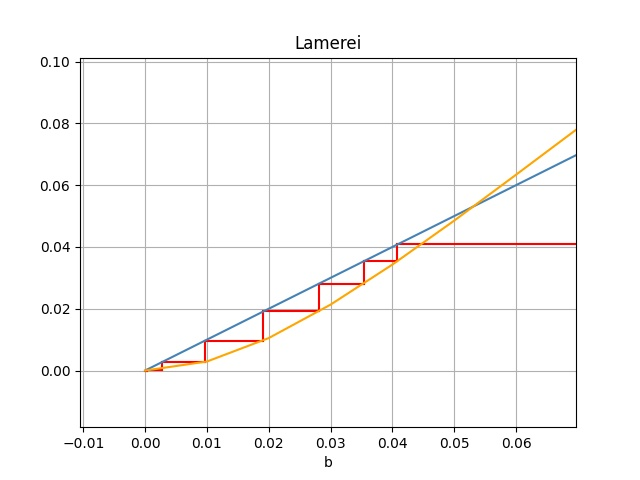
\includegraphics[width=0.75\textwidth]{lamerei2_x_1_3_b_0_56.jpg}
    
            \captionsetup{justification=centering}
            \caption{\(x_0 = 1.3\)}
            \label{lamerei2_x_1_3_b_0_56}
        \end{figure}

    \subsection{График бифуркации}

        Есть еще такой метод изучения моделей, как построение бифуркационной диаграммы. Пример такой диаграммы можно увидеть на рисунке (\ref{bifurcation}).

        \begin{figure}
            \centering
            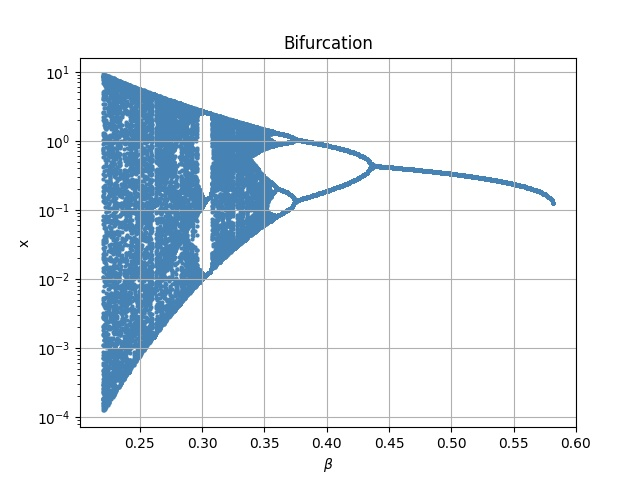
\includegraphics[width=0.75\textwidth]{bifurcation.jpg}

            \captionsetup{justification=centering}
            \caption{}
            \label{bifurcation}
        \end{figure}

        График бифуркации показывает в каком диапазоне изменяется численность популяции при конкретном значении параметра \(\beta\).

        Мы видим, что при \(\beta \in [0.44; 0.56]\) численность популяции принимает всего одно значение. Затем происходит раздвоение и при \(\beta \in [0.37; 0.44]\) видно, что есть два значения, к которым может сходится последовательность. На диапазне \(\beta \in [0.36; 0.37]\) наблюдается уже четыре возможных варианта численности популяции. 
        
        Рассмотренные выше кусочки диапазона значений \(\beta\) называются аттракторами. Чем дальше мы идем, тем зона каждого аттрактора становится все меньше и меньше. В какой-то момент начинается хаос. Когда наступает хаос уже невозможно предсказать к какому значению может сходится численность популяции.

        \comment{А может произойти деление не на две, а на три ветки?}

        \comment{Странный аттрактор}

        \comment{Книга, стр 33}

        Также на график бифуркации можно нанести линии, которые показывают границы хаоса. Такое можно увидеть на изображении (\ref{bifurcation_chaos}). Мы можем увидеть, что численность популяции не вылезает за линии границы хаоса, кроме самого начала. \comment{А вот почему я не знаю}.

        \begin{figure}
            \centering
            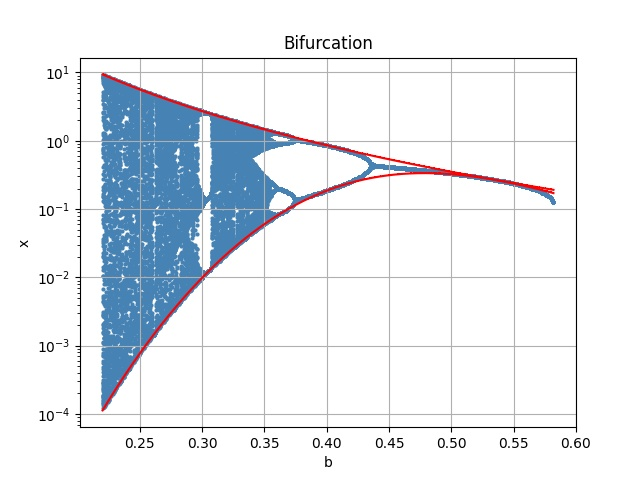
\includegraphics[width=0.75\textwidth]{bifurcation_chaos.jpg}

            \captionsetup{justification=centering}
            \caption{}
            \label{bifurcation_chaos}
        \end{figure}

    \subsection{Показатель Ляпунова}    

        Еще есть метод исследования через построение графика показателя Ляпунова. Такой график можно увидеть на рисунке (\ref{lyapunov}).

        \begin{figure}
            \centering
            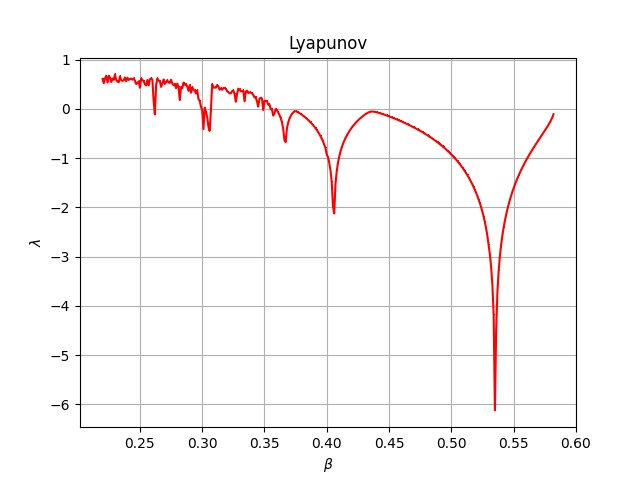
\includegraphics[width=0.75\textwidth]{lyapunov.jpg}

            \captionsetup{justification=centering}
            \caption{}
            \label{lyapunov}
        \end{figure}

        На этом графике мы видим, что точки, где график показателя Ляпунова касается нуля точно соответствуют границам аттракторов, которые мы могли наблюдать на графике бифуркации (\ref{bifurcation}).

    \subsection{Карта режимов}

        \comment{Про нее нврн вообще не стоит писать, т.к. она еще не готова. Напишем в следующем курсаче}